%&latex
%
\documentclass[../template.tex]{subfiles}
\begin{document}

\section{Diffusion with obstacles} \lesson{15}{21/11/19}
Consider a particle in a potential $U(x)$ (fig. \ref{fig:potential}), with a local minimum separated by a \textit{barrier}. In the classical case, if the particle's energy is sufficiently low, it can become \textit{forever} trapped inside the minimum. However, in the presence of \textit{thermal fluctuations} there may be a possibility of escape - a sort of classical tunnelling. 
%Sec. 5.5.3. Gardiner IV ed.

\begin{figure}[H]
    \centering
    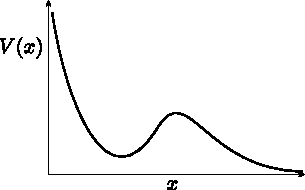
\includegraphics{Images/potential.pdf}
    \caption{Potential graph\label{fig:potential}}
\end{figure}
We first consider an easier problem, that of the diffusion process on a compact domain $[a,b]$, representing the \textit{boundaries} of the potential well of fig. \ref{fig:potential}. We then suppose that the particle cannot escape from the left side $a$, but it can do so - and always does - from the right one $b$. This means that $a$ is a \q{reflecting} boundary - i.e. if the particle hits $x=a$ it \q{bounces back}), while $x=b$ is an \textit{absorbing} boundary, that is a particle reaching $b$ can be \q{absorbed by the environment} and disappear from the system. In the more general case, the probability of reflection at $x=a$ or absorption at $x=b$ will not be certain, but will depend on the particle's energy.

\medskip

Recall the Langevin equation:
\begin{align*}
    \dd{x(t)} = \underbrace{\frac{F(x,t)}{\gamma}}_{f(x,t)}\dd{t}  + \sqrt{2D(x,t)} \dd{B} \qquad F(x) = - U'(x);\> x \in [a,b]
\end{align*}
This is equivalent to the Fokker-Planck equation:
\begin{align}\nonumber
    \pdv{t} W(x,t|x_0,0) &= -\pdv{x}\left[f(x,t) W(x,t|x_0,0) - \pdv{x} (D(x,t) W(x,t|x_0,0))\right] =\\
    &= -\pdv{x}\overbrace{\Bigg[\underbrace{-\frac{U'(x)}{\gamma}}_{A(x)}W(x,t|x_0,0) -  \pdv{x}\Big(\underbrace{\frac{k_B T}{\gamma}}_{D}   W(x,t|x_0,0)\Big)\Bigg]}^{J(x,t)} \label{eqn:fp-boundaries} =\\ \label{eqn:fp-simple}
    &= -\partial_x [A(x) W(x,t|x_0,0)] + \partial_x^2 [D(x) W(x,t|x_0,0)]
\end{align}
where we inserted $D(x,t) \equiv D =k_B T/\gamma$ (derived from the equilibrium limit). $J(x,t)$ is the probability flux coming out from $x$ at instant $t$.

To solve (\ref{eqn:fp-boundaries}) we need a precise mathematical description for the \textit{reflecting} and \textit{absorbing} boundaries:  

\begin{itemize}
    \item In $x=a$, the \textit{reflecting} boundary condition means that:
    \begin{align}
        J(a,t) = A(a)W(a,t|x_0,0) - [\partial_x D(x) W(x,t|x_0,0)]|_{x=a} \overset{!}{=}  0 \qquad \forall t
        \label{eqn:boundary-a}
    \end{align}  
    As every particle that goes in $a$ immediately comes out after being reflected, the \textit{inward} flux and \textit{outward} one are the same, and so their sum is $0$.
    \item In $b$, however, the \textit{absorbing} boundary condition means that the probability to find the particle here is exactly $0$:
    \begin{align}
        W(b,t|x_0,0) \overset{!}{=}  0 \label{eqn:boundary-b}
    \end{align}   
\end{itemize}

As $x\in [a,b]$, the domain of equation (\ref{eqn:fp-boundaries}) is not isotropic anymore - meaning that the solution $W(x,t|x_0,0)$ will depend on $x_0$, making the problem much difficult. The idea is then to translate the problem from finding the full transition probability $W(x,t|x_0,0)$ to finding a simpler, but still interesting, function, that depends on less parameters.

One possible choice is given by the \textbf{survival probability}, i.e. the probability that a particle starting at a given point $x$ will still be inside the interval $[a,b]$ at a later time $t$:
\begin{align*}
    G(x,t) = \int_a^b \dd{y} W(y,t|x,0)
\end{align*}
Note that we keep the starting time fixed at $0$, and integrate over all the possible \textit{destinations} of the particle - reducing the number of variables from $4$ to $2$.

Note that generally $G(x, t) \neq 1$, as the boundary in $b$ offers a possibility of escape, leading to a \textit{violation} of the conservation of probability. In fact the condition (\ref{eqn:boundary-b}) $W(b,t|x_0,t_0) = 0$ does not mean that the flux here is null. Recalling the definition of $J(x,t)$ from (\ref{eqn:fp-boundaries}):
\begin{align*}
    J(b,t) &= \cancel{A(b) W(b,t|x_0,t_0)} - \partial_x(D(x) W(x,t|x_0,t_0)) |_{x = b}= \\
    &= \cancel{-(\partial_x D) W(b,t|x_0,t_0) }- D(b) \partial_x W(x,t|x_0,t_0)|_{x = b} \neq 0
\end{align*}    

Now, we need to translate (\ref{eqn:fp-boundaries}) to a differential equation for $G(x,t)$. We can start by evaluating the time derivative of $G(x,t)$:
\begin{align} \label{eqn:Gtprime}
    \pdv{t} G(x,t) = \int_a^b \dd{x'} \pdv{t} W(x',t|x,0)
\end{align}
We could use (\ref{eqn:fp-simple}) to expand the $\partial_t W(x',t|x,0)$ term - but this does not really work:
\begin{align*}
    \pdv{t} G(x,t) = \int_a^b \dd{x'} [-\partial_{x'}(A(x')W(x',t|x,0)) + \partial_{x'}^2 (D(x')W(x',t|x,0))]
\end{align*}
To reconstruct derivatives of $G(x,t)$ in the right side, we would need to bring the $\partial_{x'}$ out of the integrals - but this is not possible, as $x'$ is the variable of integration. One way to solve this would be to somehow move the derivative from $\partial_{x'}$ to $\partial_x$.

To do this, we start from the ESCK relation:
\begin{align*}
    \int_a^b \dd{x_1} W(x_2, t_2|x_1,t_1) W(x_1,t_1 | x_0,t_0) = W(x_2, t_2 | x_0, t_0) \qquad t_0 < t_1 < t_2
\end{align*}
Differentiating with respect to the middle time $t_1$:
\begin{align*}
    \int_a^b \dd{x_1} [W(x_1,t_1|x_0,t_0)\partial_{t_1} W(x_2,t_2|x_1,t_1) + W(x_2,t_2|x_1,t_1)\hlc{Yellow}{ \partial_{t_1} W(x_1,t_1|x_0,t_0)]} = 0
\end{align*}
We then use (\ref{eqn:fp-simple}) to expand the highlighted term:
\begin{align*}
    &\int_a^b \dd{x_1} W(x_1,t_1|x_0,t_0)\partial_{t_1} W(x_2,t_2|x_1,t_1)+\\ \quad \>+&\int_a^b \dd{x_1} W(x_2,t_2|x_1,t_1)[-\partial_{x_1} A(x_1) W(x_1,t_1|x_0,t_0) + \partial_{x_1}^2 D(x_1)W(x_1,t_1|x_0,t_0)] = 0
\end{align*}
And then we integrate by parts the second term, to move the $\partial_{x_1}$ and $\partial_{x_1}^2$ derivatives:
\begin{align*}
    &\int_a^b \dd{x_1} W(x_1,t_1|x_0,t_0)\partial_{t_1} W(x_2,t_2|x_1,t_1)+\\
\quad \> - & A(x_1) W(x_1,t_1|x_0,t_0) W(x_2,t_2|x_1,t_1)\Big|_{x_1=a}^{x_1 = b} +W(x_2,t_2|x_1,t_1) [\partial_{x_1} D(x_1) W(x_1,t_1|x_0,t_0)] \Big|_{x_1=a}^{x_1=b}\\
\quad \> - &D(x_1)W(x_1,t_1|x_0,t_0)[\partial_{x_1} W(x_2,t_2|x_1,t_1)] \Big|_{x_1=a}^{x_1=b} \\
\quad \>+ &\int_a^b \dd{x_1} [A(x_1) W(x_1,t_1|x_0,t_0)\partial_{x_1} W(x_2,t_2|x_1,t_1) + D(x_1) W(x_1,t_1|x_0,t_0)] \partial_{x_1}^2 W(x_2,t_2|x_1,t_1) = 0
\end{align*}
In the limit $t_1 \to 0$, $W(x_1,t_1|x_0,t_0) = \delta(x_1- x_0) \delta(t_1-t_0)$. This makes all the boundary terms vanish (given that $x_0 \neq a,b$), and allows to compute the other integrals (with $x_1 = x_0$ and $t_1=t_0$), leading to:
\begin{align*}
    \pdv{t_0} W(x_2,t_2|x_0,t_0) + A(x_0) \pdv{x_0} W(x_2,t_2|x_0,t_0) + D(x_0) \pdv[2]{x_0} W(x_2,t_2|x_0,t_0) = 0
\end{align*}
Rearranging, and dropping some subscripts:
\begin{align}
    \partial_{t_0} W(x,t|x_0,t_0) = -A(x_0) \partial_{x_0} W(x,t|x_0,t_0) - D(x_0) \partial_{x_0}^2 W(x,t|x_0,t_0) \label{eqn:backward-fp}
\end{align}
This is the \textbf{backward Fokker-Planck equation}, as all derivatives are with respect to the starting time or position - meaning that it can be use to \q{retrodict} the past given the future. This could be used for computing $\partial_t G(x,t)$ - but first we need to express the derivative $\partial_{t_0}$ in terms of the derivative $\partial_t$ that appears in $\partial_t G(x,t)$.  

Supposing that $A(x)$ and $D(x)$ are time-independent (as we implicitly did in the previous notation), then (\ref{eqn:fp-simple}) is an \textit{autonomous} differential equation, meaning that the solution does not change after a time translation:
\begin{align*}
    W(x,t|x_0,t_0) = W(x,t-t_0|x_0,0)
\end{align*}  
Differentiating with respect to $t_0$:
\begin{align*}
    \partial_{t_0} W(x,t|x_0,t_0) = \partial_{t'} W(x,t'|x_0,0)|_{t' = t-t_0} \partial_{t_0}(t-t_0) = - \partial_t W(x,t-t_0|x_0,0) = -\partial_t W(x,t|x_0,t_0) 
\end{align*}
Substituting this relation in (\ref{eqn:backward-fp}) we get:
\begin{align}
    \partial_t W(x,t|x_0,t_0) = A(x_0) \partial_{x_0} W(x,t|x_0,t_0) + D(x_0) \partial_{x_0}^2 W(x,t|x_0,t_0) \label{eqn:backward-fp2}
\end{align}
Finally, we can use (\ref{eqn:backward-fp2}) in (\ref{eqn:Gtprime}):
\begin{align}
    \pdv{t}G(x,t) &= \int_a^b \dd{x'} \partial_t W(x',t|x,0) =\\ \nonumber
    &=\underset{(\ref{eqn:backward-fp2})}{=} \int_a^b \dd{x'} [A(x) \partial_x W(x',t|x,0) + D(x) \partial_{x}^2 W(x',t|x,0)] =\\ \nonumber
    &= A(x) \partial_x \underbrace{\int_a^b \dd{x'} W(x',t|x,0)}_{G(x,t)}  + D(x) \partial_{x}^2 \underbrace{\int_a^b \dd{x'} W(x',t|x,0)}_{G(x,t)} =\\
    &= A(x) \partial_x G(x,t) + D(x) \partial_{x}^2 G(x,t) \label{eqn:fpG}
\end{align}
We have now a differential equation for $G(x,t)$, and we need to translate the appropriate boundary conditions (\ref{eqn:boundary-a}) and (\ref{eqn:boundary-b}). The latter is immediate:
\begin{align}
    W(b,t|x_0,0) = 0 \qquad \forall t \> \forall x_0 \in [a,b] \Rightarrow G(x,t)|_{x=b} = 0 \label{eqn:Gboundary-b}
\end{align}
However, the analogous of (\ref{eqn:boundary-a}) requires a bit more work. So we start again from the ESCK relation, and differentiate with respect to the mid-time:
\begin{align*}
    \partial_\tau \int_a^b \dd{y} W(x',t|y, \tau) W(y, \tau|x,0) = \partial_\tau W(x',t|x,0) = 0
\end{align*}
Expanding the left side:
\begin{align*}
    \int_a^b \dd{y} [W(y, \tau|x,0)\hlc{Yellow}{ \partial_\tau W(x',t|y,\tau)} + W(x',t|y,\tau)\hlc{SkyBlue}{\partial_\tau W(y,\tau|x,0)}] = 0
\end{align*}
We can now use (\ref{eqn:backward-fp}) for the term highlighted in yellow, and (\ref{eqn:fp-simple}) (also called \textbf{forward Fokker-Planck equation}) for the term in green, leading to:
\begin{align*}
    &\int_a^b \dd{y} [-A(y) \partial_y W(x',t|y,\tau) - D(y) \partial_y^2 W(x',t|y,\tau)] W(y,\tau|x,0) +\\
    & \int_a^b \dd{y} [-\partial_y A(y) W(y,\tau|X,0) + \partial_{y}^2 D(y) W(y, \tau|x,0)] W(x',t|y,\tau)
\end{align*}
We now integrate by parts the first term, moving the $\partial_y$ and $\partial_y^2$ derivatives away from $W(x',t|y,\tau)$:
\begin{align*}
    &-A(y) W(x',t|y,\tau) W(y,\tau|x,0) \Big|_{y = a}^{y=b} +\hlc{Yellow}{ \int_a^b \dd{y} [\partial_y A(y) W(y,\tau|x,0)] W(x',t|y,\tau)} +\\
    &-D(y)W(y,\tau|x,0)[\partial_y W(x',t|y,\tau)] \Big|_{y=a}^{y=b} + W(x',t|y,\tau) [\partial_y D(y) W(y,\tau|x,0)] \Big|_{y=a}^{y=b} +\\
    &-\hlc{SkyBlue}{ \int_a^b \dd{y} [\partial_y^2 D(y) W(y,\tau|x,0)] W(x',t|y,\tau) }- \hlc{Yellow}{\int_a^b \dd{y} \partial_y [A(y) W(y,\tau|x,0)] W(x',t|y,\tau)} +\\
    &+\hlc{SkyBlue}{ \int_a^b \dd{y} \partial_y^2 [D(y) W(y,\tau|x,0)] W(x',t|y,\tau)} = 0
\end{align*}
The highlighted terms cancel out, leaving only boundaries:
\begin{align*}
    -&A(y) W(x',t|y,\tau) W(y,\tau|x,0) \Big|_{y = a} -D(y)W(y,\tau|x,0)[\partial_y W(x',t|y,\tau)] \Big|_{y=a}^{y=b} +\\
    +&W(x',t|y,\tau) [\partial_y D(y) W(y,\tau|x,0)] \Big|_{y=a}^{y=b} = 0
\end{align*}
Now $W(b,t|x_0,0) = 0$ (\ref{eqn:boundary-b}), and also $W(x',t|b,\tau) = 0$, as a particle starting in $b$ escapes immediately from $[a,b]$. This makes all the boundary terms vanish at $y=b$, leaving only:
\begin{align*}
    +&A(a) W(x',t|a,\tau) W(a,\tau|x,0) + D(a) W(a,\tau|x,0) [\partial_y W(x',t|y,\tau)] |_{y = a} +\\
    -&W(x',t|a,\tau) [\partial_y D(y) W(y, \tau|x,0)] |_{y = a} = 0
\end{align*}
Collecting $W(x',t|a,\tau)$ allows to recognize a $J(x,t)$ term:
\begin{align*}
    &D(a) W(a, \tau|x,0) [\partial_y W(x',t|y,\tau)]|_{y=a} +\\
    +& W(x',t|a,\tau) \Big[A(a) W(a,\tau|x,0) - \underbrace{[\partial_y D(y) W(y,\tau|x,0)]|_{y = a}\Big]}_{J(a,\tau)} = 0
\end{align*}
But recall that $J(a,\tau) = 0\> \forall \tau$ as per (\ref{eqn:boundary-b}). So only a term remains:
\begin{align*}
    D(a) W(a, \tau|x,0) [\partial_y W(x',t|y,\tau)]|_{y=a} = 0 \Rightarrow W(a, \tau|x,0) = 0 \> \lor \> \partial_y W(x',t|y,\tau)|_{y=a} = 0 \quad \forall \tau 
\end{align*}
Finally, by integrating the second term:
\begin{align*}
    \int_a^b \dd{x'} \partial_y W(x',t|y,\tau) = \partial_y \int_a^b \dd{x'}W(x',t|y, \tau) = \partial_y G(y, \tau)
\end{align*}
And evaluating at $y = a$ leads to:
\begin{align}
    \partial_x G(x,t) |_{x=a} = 0 \label{eqn:Gboundary-a}
\end{align}
which is the last boundary condition we needed for $G(x,t)$.

So, the problem now becomes:
\begin{align*}
    \begin{cases}
        \partial_t G(x,t) = A(x) \partial_x G(x,t) + D(x) \partial_{x}^2 G(x,t)\\
        \partial_x G(x,t)|_{x=a} = 0\\
        G(x,t)|_{x=b} = 0
    \end{cases}
\end{align*}

We can make one last simplification by \textit{removing} the time coordinate. Let's introduce $T(x)$ as being the \textit{lifetime} of a particle starting at $x$ - meaning the amount of time needed for that particle to \q{disappear} by reaching $b$ (so, in this case, $T(x)$ coincides with $T_{\mathrm{ftv}}(b,x)$, i.e. the \textit{time to the first visit} of $b$). The exact value of $T(x)$ will depend on the particle's path, making $T(x)$ a random variable. Note that:
\begin{align*}
    G(x,t) = \mathbb{P}(T(x) > t)
\end{align*}   
That is, the survival probability is the probability that the particle \textit{has not yet reached} $b$ during the time interval $[0,t]$, which is equivalent to saying that its lifetime is greater than $t$. Denoting with $\mathbb{P}_{\mathrm{ftv}}(T_b) \dd{T_b}$ the probability that a particle will visit $b$ in the time range $[T_b, T_b+\dd{T_b}]$, we have:
\begin{align*}
    G(x,t) = \mathbb{P}(T(x) > t) = \int_t^{+\infty} \mathbb{P}_{\mathrm{ftv}}(T_b) \dd{T_b} = -\int_{+\infty}^t \mathbb{P}_{\mathrm{ftv}}(T_b) \dd{T_b}
\end{align*}
Differentiating with respect to $t$:
\begin{align*}
    \partial_t G(x,t) = - \mathbb{P}_{\mathrm{fvt}}(t)
\end{align*} %Spostare sotto?

As we need a function, and $T(x)$ is a random variable, we consider its \textit{average}, i.e. the \textit{mean time of arrival at $b$} $T_b(x)$: 
\begin{align} \nonumber
    T_b(x) &\equiv \langle T(x) \rangle \equiv \int_0^{+\infty} t \mathbb{P}_{\mathrm{fvt}}(t) \dd{t} = -\int_0^{+\infty} t \partial_t G(x,t) \dd{t} =\\
    &= -t G(x,t)\Big|_{t=0}^{t=+\infty} + \int_0^{+\infty} G(x,t) \dd{t} \underset{(a)}{=} \langle G(x) \rangle \label{eqn:Gavg}
\end{align} 
In (a) we used that $t G(x,t)$ vanishes at $t=0$ and also at $t=+\infty$, because the particle will eventually reach $x=b$ if given infinite time to do so. It is not clear if $G(x,t)  \xrightarrow[t \to \infty]{}   0$ \textit{faster} than $t \to \infty$, so that $t G(x,t)  \xrightarrow[t \to \infty]{} 0$. Here, we will just assume it, as it is physically reasonable.

\medskip

Then, we need to translate once again everything to expressions involving $T_b(x)$. Fortunately, this time it is much quicker. To get the differential equation, we just integrate (\ref{eqn:fpG}):
\begin{align*}
    \int_{0}^{+\infty} \dd{t} \partial_t G(x,t) = A(x) \partial_x \int_0^{+\infty} G(x,t) \dd{t} + D(x) \partial_x^2 \int_0^{+\infty} G(x,t) \dd{t}
\end{align*}
And applying (\ref{eqn:Gavg}) we get:
\begin{align*}
    G(x,t)\Big|_{t=0}^{t=+\infty} = G(x,+\infty) - G(x,0) = -1 = A(x) \partial_x T_b(x) + D(x) \partial_x^2 T_b(x)
\end{align*}
as $G(x,+\infty) = 0$ (no particle lives eternally) and $G(x,0) = 0$ (as a particle does not \q{disappear} immediately for $x\neq b$). Similarly, integrating (\ref{eqn:Gboundary-a}) and (\ref{eqn:Gboundary-b}) leads to:
\begin{align*}
    \begin{cases}
        A(x) \partial_x T_b(x) + D(x) \partial_x^2 T_b(x) = -1\\
        T_b(x)|_{x=b} = 0\\
        \partial_x T_b(x) |_{x=a} = 0
    \end{cases}
\end{align*} 
This is a linear ordinary differential equation. We start by letting $f(x) = \partial_x T_b(x)$, leading to:
\begin{align*}
    f'(x) = - \frac{A(x)}{D(x)} f(x) - \frac{1}{D(x)} \qquad f(a) = 0 
\end{align*}
First consider the \textit{homogeneous} equation:
\begin{align*}
    A(x) \Phi(x) + D(x) \Phi'(x) = 0
\end{align*} 
This can be solved by separation of variables:
\begin{align*}
    Af + D\dv{\Phi}{x} = 0 \Rightarrow \frac{\dd{\Phi}}{\Phi} = - \frac{A}{D} \dd{x} \Rightarrow \ln |\Phi(x)| = -\int_{x_0}^x \frac{A(y)}{D(y)} \dd{y} + c
\end{align*}
where $x_0$ is a fixed point $\in [a,b]$ (it does not matter which one).
Exponentiating: 
\begin{align*}
    \Phi(x) = \exp\left(-\int_{x_0}^x \frac{A(y)}{D(y)}\dd{y} \right) k
\end{align*}
Where $k = e^c$ will be fixed by the boundary condition $f(a) = 0$. First, we need to find the general integral of the inhomogeneous equation - for example by using the method of \textbf{variation of parameters}.

\begin{expl}\textbf{Refresher of variation of parameters}. Consider the following Cauchy problem:
    \begin{align*}
        \begin{cases}
            y' = A(t) y + b(t)\\
            y(t_0) = y_0
        \end{cases}
    \end{align*}
    Suppose we know a solution $\Phi(t)$ of the homogeneous equation $y'=A(t)y$. Then $\Phi' = A \Phi$. We search for a particular solution for the full equation in the form $\tilde{\varphi}(t) = \Phi(t) c(t)$. Substituting in the equation:
    \begin{align*}
        \Phi' c + c' \Phi = A \Phi c + c' \Phi = A \Phi c + b \Rightarrow c' = \Phi^{-1} b 
    \end{align*}
    This can be integrated to find $c$, and then $\tilde{\varphi}$. 
    Then, the general integral will be the sum of the homogeneous solution $\Phi(t)$ and the particular one $\tilde{\varphi}$. Imposing the boundary condition will lead to the general integral:
    \begin{align}\label{eqn:general-integral}
        \varphi(t) = \Phi(t) \Phi(t_0)^{-1} y_0 + \Phi(t) \int_{t_0}^t \Phi(\tau)^{-1} b(\tau) \dd{\tau}
    \end{align}
\end{expl}
Applying formula (\ref{eqn:general-integral}) leads to the desired $f(x)$:
\begin{align*}
    f(x) &= \Phi(x) \Phi(a) \cdot 0 + \Phi(x) \int_a^x \dd{z} \Phi(z)^{-1} \left[-\frac{1}{D(z)} \right] =\\
    &= \exp\left(-\int_{x_0}^x \frac{A(y)}{D(y)} \dd{y} \right) \int_a^x -\frac{\dd{z}}{D(z)}  \exp\left(+\int_{x_0}^z \frac{A(y)}{D(y)}\dd{y} \right) =\\
    &= - \int_a^x \frac{\dd{z}}{D(z)} \exp\left(+\int_x^z \frac{A(y)}{D(y)}\dd{y} \right) 
\end{align*}
Recall that $f(x) = \partial_x T_b(x)$, with $T_b(b) = 0$. So, to find $T_b(x)$ we need one last integration:
\begin{align*}
    T_b(x) = \int_{x_0}^x \dd{y} f(y) + c
\end{align*}
Imposing $T_b(b) = 0$ leads to:
\begin{align*}
    T_b(b) = \int_{x_0}^b \dd{y} f(y) + c \overset{!}{=} 0 \Rightarrow c = -\int_{x_0}^b \dd{y} f(y)
\end{align*}
Leading to:
\begin{align}
    T_b(x) =\int_b^x \dd{y} f(y) = \int_x^b \dd{y} \int_a^y \frac{\dd{z}}{D(z)} \exp\left(-\int_z^y \dd{v}\frac{A(v)}{D(v)} \right) 
    \label{eqn:sol1}
\end{align}

\subsection{Escape from a potential well}
Let's now use (\ref{eqn:sol1}) to solve the problem we started from. So, suppose to have a potential $U(x)$ with a local minimum at $x=c$, and a local maximum at $x=d$, with $c < d$. Consider a particle starting at $x=c$. We wish to compute the average first visit time of $d$, denoted with $\langle T(c \to d) \rangle$. 
This can be done by redefining the system as the half-line $[-\infty,d]$, with $x=-\infty$ being a \textit{reflective} boundary, and $x=d$ an \textit{absorbing} one. We can do this because we are not interested in the behaviour \textit{after} passing $d$, but just in the mean arrival times.

So $A(x) = - \partial_x U(x)/\gamma$. Supposing to be at equilibrium, $D(x) \equiv D = 1/(\gamma B)$. Letting $a=-\infty$ and $b=d$ leads to:
\begin{align*}
    T_d(x) &= \int_x^d \dd{y} \int_{-\infty}^y \beta \gamma \dd{z} \exp\left(-\int_z^y -\dd{v}\frac{\partial_v U(v)}{\gamma} \gamma \beta \right) =\\
    &= \beta \gamma \int_x^d \dd{y} \int_{-\infty}^{y} \dd{z} \exp(\beta [U(y) - U(z)]) =\\
    &= \beta \gamma \int_x^d \dd{y} e^{\beta U(y)} \underbrace{\int_{-\infty}^{y} \dd{z} e^{- \beta U(z)}}_{e^{F(y)}}  = \beta \gamma \int_x^{d} \dd{y} e^{\beta U(y) + F(y)}
\end{align*}
It is not possible to evaluate this integral in the general case. However, in the limit $\beta \to \infty$ ($T \to 0$) we can use the saddle-point approximation. 

Recall Laplace's formula:
\begin{align*}
    \int_a^b e^{M f(x)} \dd{x} \underset{M \to +\infty}{\approx}  \sqrt{\frac{2 \pi}{M|f''(x_0)|} } e^{Mf(x_0)}
\end{align*}
where $f'(x_0) = 0$ and $f''(x_0) < 0$.

For the integral in $\dd{z}$, $f(z) = -U(z)$. We search for a maximum of $f(z)$, i.e. a minimum of $U(z)$, which is $z=c$. So:
\begin{align*}
    \int_{-\infty}^y e^{- \beta U(z) }\dd{z} = \sqrt{\frac{2 \pi}{\beta U''(c)}} e^{-\beta U(c)}  
\end{align*}
This is a constant, and can be brought outside the integral over $\dd{y}$. Then, by applying Laplace's formula once again:
\begin{align*}
    \int_c^d \dd{y} e^{\beta U(y)} = \sqrt{\frac{2 \pi}{\beta |U''(d)|} } e^{\beta U(d)}
\end{align*}
as now $f(y) = U(y)$, and $U$ has a local maximum in $y = d$. Finally, this leads to:
\begin{align*}
    T_d(c) \underset{T \to 0}{\approx}  \frac{2 \pi \gamma}{\sqrt{U''(c) |U''(d)|}}  \exp\left(\beta[U(d) - U(c)]\right)
\end{align*}
Note that the mean transition time from $c$ to $d$ diverges exponentially as the barrier's height $U(d) - U(c)$ rises. Equivalently, the \textit{escape transition rate} $1/T_d(c) \to 0$.  


\section{Feynman Path Integral}
We finish our discussion about the diffusion formalism noting several correspondences with quantum processes.

Recall the Sch\"odinger equation:
\begin{align*}
    i \hbar \pdv{t} \psi(x,t) &= - \frac{\hbar^2}{2 m} \pdv[2]{x} \psi(x,t) + V(x) \psi(x,t) =\\
    &= H(x, \partial_x^2,t) \psi(x,t)
\end{align*}
where $H$ is the \textit{Hamiltonian} operator:
\begin{align*}
    H(x, \partial_x^2,t) \equiv -\frac{\hbar^2}{2m} \partial_x^2 + V(x,t) 
\end{align*}  
If we consider a free particle ($V(x,t) \equiv 0$), the Schr\"odinger equation becomes:
\begin{align}
    \partial_t \psi = i \frac{\hbar}{2m} \partial_x^2 \psi  \qquad \psi(x,0) = \delta(x-x_0) \label{eqn:schrody}
\end{align}
which is very similar to the diffusion equation:
\begin{align}\label{eqn:dif}
    \partial_t W(x,t) = D\partial_x W(x,t) \qquad W(x,t|x_0,0) \Big|_{t=0} = \delta(x-x_0)
\end{align}
In fact, we can map (\ref{eqn:schrody}) to (\ref{eqn:dif}) by defining a \textit{quantum diffusion coefficient} $D_{QM} = i \hbar/(2m)$.

\medskip

Does this mean that all properties of the diffusion equation - and its solution - can be mapped to the quantum case? Unfortunately, the answer is a bit complex.

Recall that the solution of (\ref{eqn:dif}) for a particle initially starting in $x_0$ at $t_0$ is:
\begin{align} \label{eqn:dif-sol}
    W(x,t|x_0,t_0) = \frac{1}{\sqrt{4 \pi D (t-t_0)}} \exp\left(-\frac{(x - x_0)^2}{4 D (t-t_0)} \right) 
\end{align}
By substituting $D \leftrightarrow D_{\mathrm{QM}}$ we can construct the analogous \textit{quantum} solution:
\begin{align} \label{eqn:schrody-sol}
    \psi(x,t) = \sqrt{\frac{2m}{4 \pi (t-t_0)i \hbar} } \exp\left(i \frac{m}{2\hbar} \frac{(x-x_0)^2}{t-t_0}  \right) 
\end{align} 
Note that now the exponential argument is \textit{complex}, making basic properties of (\ref{eqn:dif-sol}) not-trivial. For example, if $t \to t_0$, the exponential in (\ref{eqn:dif-sol}) tends to a $\delta$:
\begin{align*}
    \lim_{t \to t_0} W(x,t|x_0,t_0) = \delta(x-x_0)
\end{align*}
giving back the starting distribution, as expected.

The same, however, does not happen for (\ref{eqn:schrody-sol}), given the presence of the $i$. Nonetheless, it is true that in the limit $t \to t_0$, (\ref{eqn:schrody-sol}) is a \textit{infinitely oscillating function}, meaning that it is $0$ \textit{almost} everywhere. This can be proven by using more sophisticated techniques, such as the \textit{stationary phase approximation}. 

\medskip

What about path integrals? If we start with the usual definition and make the substitution $D \leftrightarrow D_{\mathrm{QM}}$ we get:
\begin{align*}
    \psi(x,t) &= \langle \delta(x(t) - x) \rangle_W =\\
    &= \int_{\mathbb{R}^T} \prod_{\tau = 0^+}^t \frac{\dd{x(\tau)}}{\sqrt{4 \pi D_\mathrm{QM}} \dd{\tau}} \exp\left(-\frac{1}{4 D_{\mathrm{QM}}} \int_0^t \left(\dv{x(\tau)}{\tau}\right)^2 \dd{\tau} \right) \delta(x(t)-x) =\\
&= \int_{\mathbb{R}^T} \prod_{\tau = 0^+}^t \frac{\dd{x(\tau)}}{\sqrt{4 \pi D_{QM} \dd{t}}} \exp\left(\frac{\textcolor{Red}{i}}{\hbar} \frac{1}{2}m \int_0^t \left[\dv{x(\tau)}{\tau}\right]^2 \dd{\tau} \right) \delta(x(t)-x)
\end{align*}
Note that now \textit{trajectories} are weighted by a \textit{complex number}. This means that they \textit{are not probabilities} - and in particular, we cannot use Kolmogorov extension theorem to prove the existence of such a measure as the \textit{continuum limit} of a measure defined on \textit{discretized paths}.

However, we note that in the limit $\hbar \to 0$, the integral can be approximated with the saddle-point method, which returns the \textit{classical trajectory} - the one where the \textit{phases oscillate slowly}.

In fact, it can be proven that \textit{QM} cannot be derived by statistical mechanics alone: quantum \q{noise} is very much different from thermal \q{noise}!

\medskip

Consider now the more general case of non-zero potential:
\begin{align*}
    \pdv{t} \psi(x,t) = i \frac{\hbar}{2m} \partial_x^2 \psi(x,t) - \frac{iV(x)}{\hbar} \psi(x,t)   
\end{align*}
which is just the quantum evaluated version of the Fokker-Planck equation:
\begin{align*}
    \partial_t W(x,t) = D \partial_x^2 W(x,t) - V(x) W(x,t)
\end{align*}
with the substitutions:
\begin{align} \label{eqn:qtm-subs}
    D &\to D_{QM} = \frac{i \hbar}{2m}\\ \nonumber
    V &\to \frac{i}{\hbar}V  
\end{align}
The solution we obtained from discussing the diffusion process is:
\begin{align*}
    W(x,t|x_0,t_0) &= \langle \exp\left(-\int_0^t V(x(\tau))\dd{\tau}\right) \delta(x(t)-x)\rangle_W = \\
    &= \int_{\mathbb{R}^T} \prod_{\tau = 0^+}^t \frac{\dd{x(\tau)}}{\sqrt{4 D \pi} \dd{\tau}} \exp\left(-\frac{1}{4D} \int_0^t \dot{x}^2(\tau) \dd{\tau} - \int_0^t V(x(\tau))\dd{\tau} \right) \delta(x(t)-x)
\end{align*}
Applying (\ref{eqn:qtm-subs}) we arrive to the \textbf{Feynman path integral}: 
\begin{align*} \label{eqn:feynman-path}
    \psi(x,t) = \int_{\mathbb{R}^T} \prod_{\tau = 0^+}^t \frac{\dd{x(\tau)}}{\sqrt{4 \pi D_{QM}}\dd{\tau}}\exp\Big(\frac{i}{\hbar} \int_0^t \dd{\tau} \underbrace{\left[\frac{\dot{x}^2(\tau)}{2} - V(x(\tau)) \right]}_{L(\dot{x},x)}  \Big)  \delta(x(t)-x)
\end{align*}
To compute it we can resort to variational methods. We define the action functional $S$ as: 
\begin{align*}
    S \equiv \int_0^t \dd{\tau} L(\dot{x}(\tau), x(\tau))
\end{align*} 
Note that the Feynman path integral \textit{weights} every trajectory with the following quantity:
\begin{align*}
    \exp\left(\frac{i}{\hbar} S\left(\{x(\tau)\}_{\tau\in[0,t]}\right) \right)
\end{align*} 
Then, according to the variational method, we can approximate $\psi(x,t)$ by evaluating it only for the \textit{most contributing trajectory}, i.e. the one that \textit{stationarizes} $S$: $\delta S = 0$, implying:
\begin{align*}
    x_c \colon 
    \pdv{L}{x} - \dv{t} \pdv{L}{\dot{x}} \Big|_{x_c} = 0
\end{align*}     

\end{document}
